
This tutorial will guide you through a typical \code{pymc} application.
Familiarity with Python is assumed, so if you are new to Python, books such as
\citet{Lutz:2007} or \citet{Langtangen:2009} are the place to start. Plenty of
online documentation can also be found on the
\href{http://www.python.org/doc/}{Python documentation} page.

\section{An example statistical model}
Consider the following dataset, which is a time series of recorded coal mining
disasters in the UK from 1851 to 1962 \citep{Jarrett:1979fr}.
\begin{center}
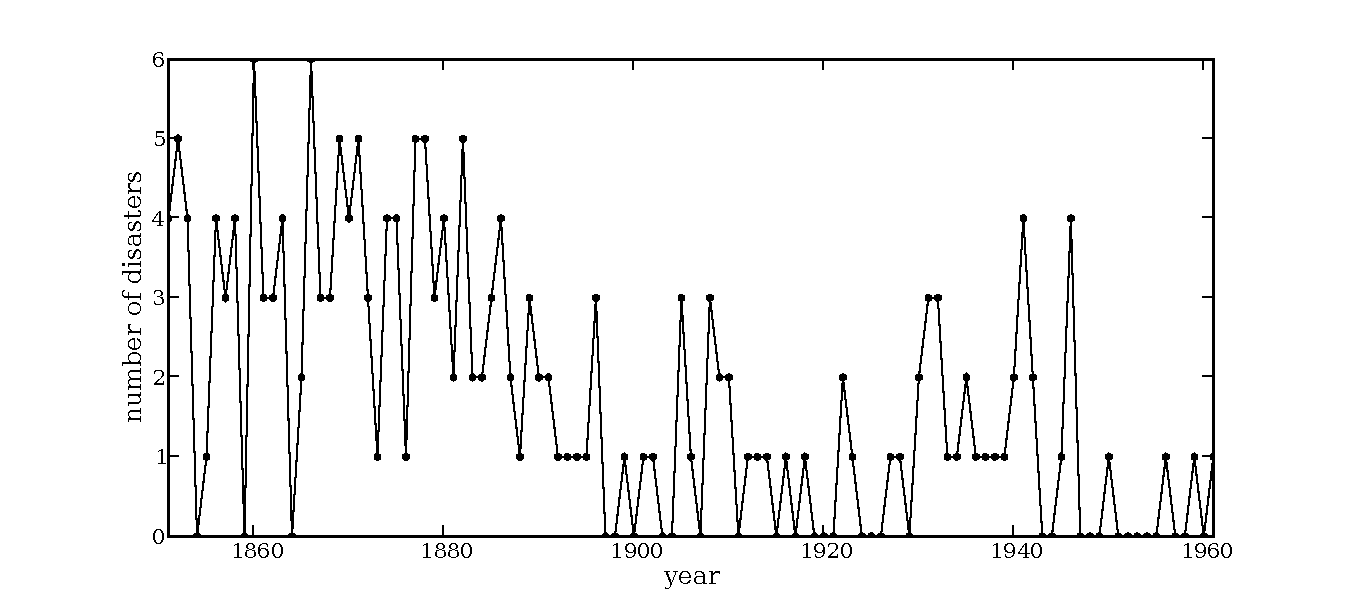
\epsfig{file=disasterts.pdf, width=15cm}
\end{center}
Occurrences of disasters in the time series is thought to be derived from a Poisson process with a large rate parameter in the early part of the time series, and from one with a smaller rate in the later part. We are interested in locating the change point in the series, which perhaps is related to changes in mining safety regulations.

We represent our conceptual model formally as a statistical model:
\begin{equation}
    \begin{array}{ccc}
        (D_t | s, e, l) \sim \textup{Poisson}\left(r_t\right), & r_t=\left\{\begin{array}{lll}
            e &\textup{if}& t< s\\ l &\textup{if}& t\ge s
            \end{array}\right.,&t\in[t_l,t_h]\\
        s\sim \textup{Discrete Uniform}(t_l, t_h)\\
        e\sim \textup{Exponential}(r_e)\\
        l\sim \textup{Exponential}(r_l)
    \end{array}
    \label{disastermodel}
\end{equation}
The symbols are defined as:
\begin{description}
    \item[$D_t$:] The number of disasters in year $t$.
    \item[$r_t$:] The rate parameter of the Poisson distribution of disasters in year $t$.
    \item[$s$:] The year in which the rate parameter changes (the switchpoint).
    \item[$e$:] The rate parameter before the switchpoint $s$.
    \item[$l$:] The rate parameter after the switchpoint $s$.
    \item[$t_l$, $t_h$:] The lower and upper boundaries of year $t$.
    \item[$r_e$, $r_l$:] The rate parameters of the priors of the early and late rates, respectively.
    %\item[$\beta_e$, $\beta_l$:] Prior parameters (also called hyperparameters).
\end{description}
Because we have defined $D$ by its dependence on $s$, $e$ and $l$, the latter three are known as the `parents' of $D$ and $D$ is called their `child'. Similarly, the parents of $s$ are $t_l$ and $t_h$, and $s$ is the child of $t_l$ and $t_h$.


\section{Two types of variables}

At the model-specification stage (before the data are observed), $D$, $s$, $e$,
$r$ and $l$ are all random variables. Bayesian `random' variables have not
necessarily arisen from a physical random process. The Bayesian interpretation
of probability is \emph{epistemic}, meaning random variable $x$'s probability
distribution $p(x)$ represents our knowledge and uncertainty about $x$'s value
\citep{jaynes}. Candidate values of $x$ for which $p(x)$ is high are
relatively more probable, given what we know. Random variables are represented
in PyMC by the classes \code{Stochastic} and \code{Deterministic}.

The only \code{Deterministic} in the model is $r$. If we knew the values of
$r$'s parents ($s$, $l$ and $e$), we could compute the value of $r$ exactly. A
\code{Deterministic} like $r$ is defined by a mathematical function that returns
its value given values for its parents. \code{Deterministic} variables are
sometimes called the \emph{systemic} part of the model. The nomenclature is a
bit confusing, because these objects usually represent random variables; since
the parents of $r$ are random, $r$ is random also. A more descriptive (though
more awkward) name for this class would be \code{DeterminedByValuesOfParents}.

On the other hand, even if the values of the parents of variables $s$, $D$ (before observing the data), $e$ or $l$ were known, we would still be uncertain of their values. These variables are characterized by probability distributions that express how plausible their candidate values are, given values for their parents. The \code{Stochastic} class represents these variables. A more descriptive name for these objects might be \code{RandomEvenGivenValuesOfParents}.

We can represent model \ref{disastermodel} in a file called
\module{DisasterModel.py} (the actual file can be found in
\file{pymc/examples/}) as follows. First, we import the PyMC and NumPy
namespaces:
\begin{verbatim}
	from pymc import DiscreteUniform, Exponential, deterministic, Poisson, Uniform
	import numpy as np
\end{verbatim}
Notice that from \code{pymc} we have only imported a select few objects that are needed for this particular model, whereas the entire \code{numpy} namespace has been imported, and conveniently given a shorter name. Objects from NumPy are subsequently accessed by prefixing \code{np.} to the name. Either approach is acceptable.

Next, we enter the actual data values into an array:
\begin{verbatim}
	disasters_array =   np.array([ 4, 5, 4, 0, 1, 4, 3, 4, 0, 6, 3, 3, 4, 0, 2, 6,
	                   3, 3, 5, 4, 5, 3, 1, 4, 4, 1, 5, 5, 3, 4, 2, 5,
	                   2, 2, 3, 4, 2, 1, 3, 2, 2, 1, 1, 1, 1, 3, 0, 0,
	                   1, 0, 1, 1, 0, 0, 3, 1, 0, 3, 2, 2, 0, 1, 1, 1,
	                   0, 1, 0, 1, 0, 0, 0, 2, 1, 0, 0, 0, 1, 1, 0, 2,
	                   3, 3, 1, 1, 2, 1, 1, 1, 1, 2, 4, 2, 0, 0, 1, 4,
	                   0, 0, 0, 1, 0, 0, 0, 0, 0, 1, 0, 0, 1, 0, 1])
\end{verbatim}
Note that you don't have to type in this entire array to follow along; the code is available in the source tree, in \file{pymc/examples/DisasterModel.py}.  Next, we create the switchpoint variable $s$:
\begin{verbatim}
	s = DiscreteUniform('s', lower=0, upper=110, doc='Switchpoint[year]')
\end{verbatim}
\code{DiscreteUniform} is a subclass of \code{Stochastic} that represents uniformly-distributed discrete variables. Use of this distribution suggests that we have no preference \emph{a priori} regarding the location of the switchpoint; all values are equally likely. Now we create the exponentially-distributed variables $e$ and $l$ for the early and late Poisson rates, respectively:
\begin{verbatim}
	e = Exponential('e', beta=1)
	l = Exponential('l', beta=1)
\end{verbatim}
Next, we define the variable $r$, which selects the early rate $e$ for times before $s$ and the late rate $l$ for times after $s$. We create $r$ using the \code{deterministic} decorator, which converts the ordinary Python function $r$ into a \code{Deterministic} object.
\begin{verbatim}
	@deterministic(plot=False)
	def r(s=s, e=e, l=l):
		""" Concatenate Poisson means """
	    out = np.empty(len(disasters_array))
	    out[:s] = e
	    out[s:] = l
	    return out
\end{verbatim}
The last step is to define the number of disasters $D$. This is a stochastic variable, but unlike $s$, $e$ and $l$ we have observed its value. To express this, we set the argument \code{observed} to \code{True} (it is set to \code{False} by default). This tells PyMC that this object's value should not be changed:
\begin{verbatim}
	D = Poisson('D', mu=r, value=disasters_array, observed=True)
\end{verbatim}

\subsection{Why are data and unknown variables represented by the same
object?}
Since its represented by a \code{Stochastic} object, $D$ is defined by its dependence on its parent $r$ even though its value is fixed. This isn't just a quirk of PyMC's syntax; Bayesian hierarchical notation itself makes no distinction between random variables and data. The reason is simple: to use Bayes' theorem to compute the posterior $p(e,s,l|D)$ of model \ref{disastermodel}, we require the likelihood $p(D|e,s,l)$. Even though $D$'s value is known and fixed, we need to formally assign it a probability distribution as if it were a random variable. Remember, the likelihood and the probability function are essentially the same, except that the former is regarded as a function of the parameters and the latter as a function of the data.

This point can be counterintuitive at first, as many peoples' instinct is to regard data as fixed a priori and unknown variables as dependent on the data. One way to understand this is to think of statistical models like (\ref{disastermodel}) as predictive models for data, or as models of the processes that gave rise to data. Before observing the value of $D$, we could have sampled from its prior predictive distribution $p(D)$ (\emph{i.e.} the marginal distribution of the data) as follows:
\begin{enumerate}
    \item Sample $e$, $s$ and $l$ from their priors.
    \item Sample $D$ conditional on these values.
\end{enumerate}
Even after we observe the value of $D$, we need to use this process model to make inferences about $e$, $s$ and $l$ because its the only information we have about how the variables are related.

% ==================================
% = Does this section really help? =
% ==================================
% \medskip
% To look at the issue another way, we could, in principle, have written a model equivalent to (\ref{disastermodel}) such that $D$ depended on nothing and everything else depended on $D$, for example
% \begin{eqnarray*}
%     s|e,l,D\sim\cdot\\
%     e|l,D\sim\cdot\\
%     l|D\sim\cdot\\
%     D=D_*
% \end{eqnarray*}
%
% In one respect, this would have been more natural because we would have the unknown stochastic variables depending on the data. However, if we could write down that model using standard distributions we could trivially compute and sample from the posterior,
% \begin{eqnarray*}
%     p(s,e,l|D) = p(s|e, l, D) p(e|l, D) p(l|D),
% \end{eqnarray*}
% and we would have no use for MCMC or any other fitting method. Bayesian methods, and statistics in general, are needed when it's feasible to write down the data's dependence on the unknown variables but not vice versa.


\section{Parents and children}

We have above created a PyMC probability model, which is simply a linked collection of variables. To see the nature of the links, import or run \code{DisasterModel.py} and examine $s$'s \code{parents} attribute from the Python prompt:
\begin{verbatim}
   >>> from pymc.examples import DisasterModel
   >>> DisasterModel.s.parents
   >>> {'lower': 0, 'upper': 110}
\end{verbatim}
The \code{parents} dictionary shows us the distributional parameters of $s$, which are constants. Now let's examinine $D$'s parents:
\begin{verbatim}
   >>> DisasterModel.D.parents
   >>> {'mu': <pymc.PyMCObjects.Deterministic 'r' at 0x3e51a70>}
\end{verbatim}
We are using $r$ as a distributional parameter of $D$ (\emph{i.e.} $r$ is $D$'s parent). $D$ internally labels $r$ as \code{mu}, meaning $r$ plays the role of the rate parameter in $D$'s Poisson distribution. Now examine $r$'s \code{children} attribute:
\begin{verbatim}
   >>> DisasterModel.r.children
   >>> set([<pymc.distributions.Poisson 'D' at 0x3e51290>])
\end{verbatim}
Because $D$ considers $r$ its parent, $r$ considers $D$ its child. Unlike \code{parents}, \code{children} is a set (an unordered collection of objects); variables do not associate their children with any particular distributional role. Try examining the \code{parents} and \code{children} attributes of the other parameters in the model.

The following `directed acyclic graph' is a visualization of the parent-child relationships in the model. Unobserved stochastic variables $s$, $e$ and $l$ are open ellipses, observed stochastic variable $D$ is a filled ellipse and deterministic variable $r$ is a triangle. Arrows point from parent to child and display the label that the child assigns to the parent. See section \ref{graphical} for more details.
\begin{center}
   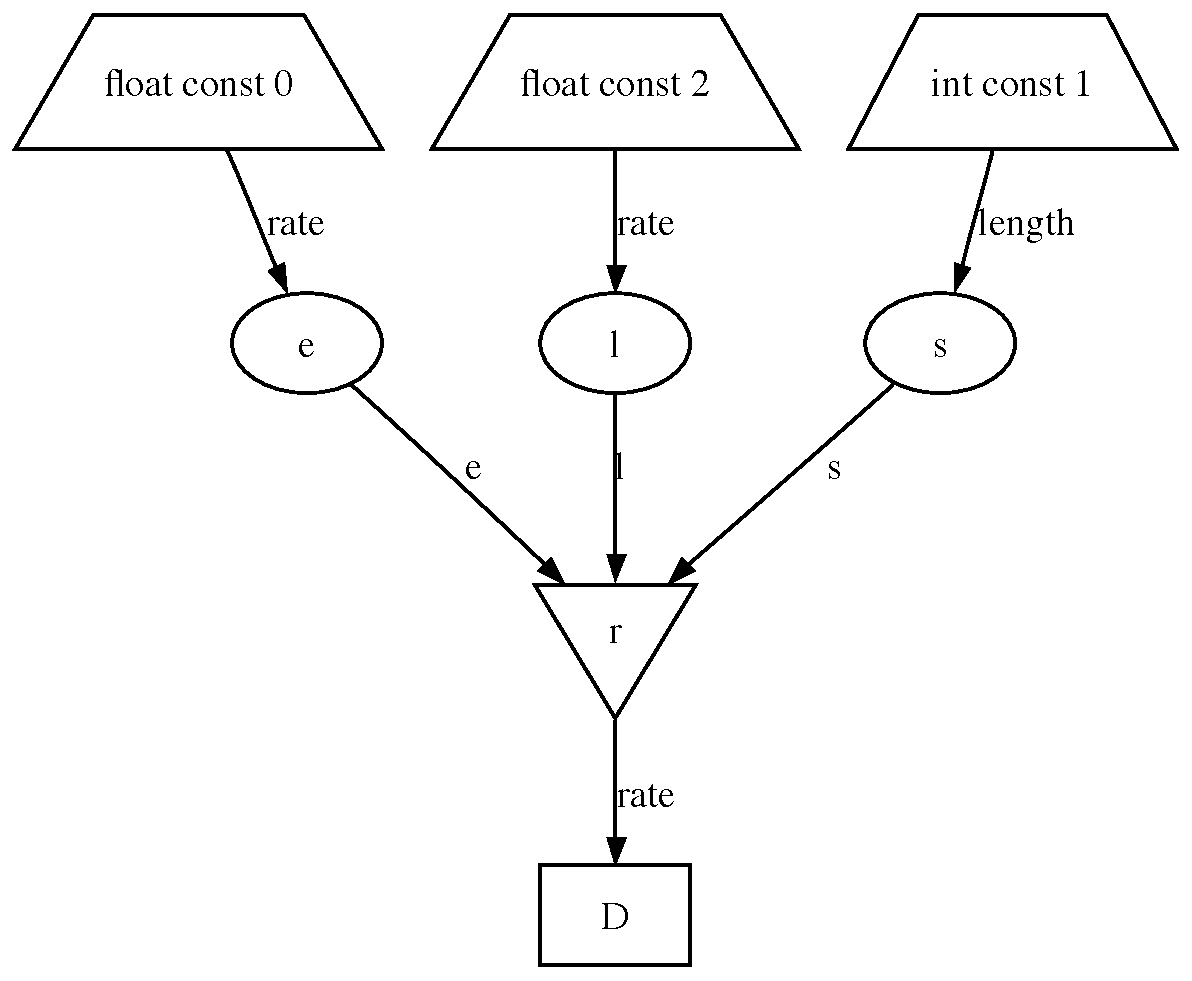
\epsfig{file=DisasterModel2.pdf, width=5cm}
\end{center}


\begin{center}
\begin{sffamily}
\fbox{\parbox{\admonitionwidth}{
\textbf{\large Objects and names}
\vspace{2mm}
As the examples above have shown, pymc objects need to have a name 
assigned, such as \emph{lower}, \emph{upper} or \emph{e}. These names 
are used for storage and post-processing:
\begin{itemize}
 \item as keys in on-disk databases,
 \item as node labels in model graphs,
 \item as axis labels in plots of traces, 
 \item as table labels in summary statistics. 
\end{itemize}
A model instantiated with variables having identical names raises an
error to avoid name conflicts in the database storing the traces. In
general however, pymc uses references to the objects themselves, not 
their names, to identify variables. 
}}
\end{sffamily}
\end{center}



\section{Variables' values and log-probabilities}
All PyMC variables have an attribute called \code{value} that stores the current value of that variable. Try examining $D$'s value, and you'll see the initial value we provided for it:
\begin{verbatim}
   >>> DisasterModel.D.value
   >>>
   array([4, 5, 4, 0, 1, 4, 3, 4, 0, 6, 3, 3, 4, 0, 2, 6, 3, 3, 5, 4, 5, 3, 1,
          4, 4, 1, 5, 5, 3, 4, 2, 5, 2, 2, 3, 4, 2, 1, 3, 2, 2, 1, 1, 1, 1, 3,
          0, 0, 1, 0, 1, 1, 0, 0, 3, 1, 0, 3, 2, 2, 0, 1, 1, 1, 0, 1, 0, 1, 0,
          0, 0, 2, 1, 0, 0, 0, 1, 1, 0, 2, 3, 3, 1, 1, 2, 1, 1, 1, 1, 2, 4, 2,
          0, 0, 1, 4, 0, 0, 0, 1, 0, 0, 0, 0, 0, 1, 0, 0, 1, 0, 1])
\end{verbatim}
If you check $e$'s, $s$'s and $l$'s values, you'll see random initial values generated by PyMC:
\begin{verbatim}
   >>> DisasterModel.s.value
   >>> 44

   >>> DisasterModel.e.value
   >>> 0.33464706250079584

   >>> DisasterModel.l.value
   >>> 2.6491936762267811
\end{verbatim}
Of course, since these are \code{Stochastic} elements, your values will be different than these. If you check $r$'s value, you'll see an array whose first $s$ elements are $e$ (here 0.33464706), and whose remaining elements are $l$ (here 2.64919368):
\begin{verbatim}
   >>> DisasterModel.r.value
   >>>
   array([ 0.33464706,  0.33464706,  0.33464706,  0.33464706,  0.33464706,
           0.33464706,  0.33464706,  0.33464706,  0.33464706,  0.33464706,
           0.33464706,  0.33464706,  0.33464706,  0.33464706,  0.33464706,
           0.33464706,  0.33464706,  0.33464706,  0.33464706,  0.33464706,
           0.33464706,  0.33464706,  0.33464706,  0.33464706,  0.33464706,
           0.33464706,  0.33464706,  0.33464706,  0.33464706,  0.33464706,
           0.33464706,  0.33464706,  0.33464706,  0.33464706,  0.33464706,
           0.33464706,  0.33464706,  0.33464706,  0.33464706,  0.33464706,
           0.33464706,  0.33464706,  0.33464706,  0.33464706,  2.64919368,
           2.64919368,  2.64919368,  2.64919368,  2.64919368,  2.64919368,
           2.64919368,  2.64919368,  2.64919368,  2.64919368,  2.64919368,
           2.64919368,  2.64919368,  2.64919368,  2.64919368,  2.64919368,
           2.64919368,  2.64919368,  2.64919368,  2.64919368,  2.64919368,
           2.64919368,  2.64919368,  2.64919368,  2.64919368,  2.64919368,
           2.64919368,  2.64919368,  2.64919368,  2.64919368,  2.64919368,
           2.64919368,  2.64919368,  2.64919368,  2.64919368,  2.64919368,
           2.64919368,  2.64919368,  2.64919368,  2.64919368,  2.64919368,
           2.64919368,  2.64919368,  2.64919368,  2.64919368,  2.64919368,
           2.64919368,  2.64919368,  2.64919368,  2.64919368,  2.64919368,
           2.64919368,  2.64919368,  2.64919368,  2.64919368,  2.64919368,
           2.64919368,  2.64919368,  2.64919368,  2.64919368,  2.64919368,
           2.64919368,  2.64919368,  2.64919368,  2.64919368,  2.64919368])
\end{verbatim}
To compute its value, $r$ calls the funtion we used to create it, passing in the values of its parents.

\code{Stochastic} objects can evaluate their probability mass or density functions at their current values given the values of their parents. The logarithm of a stochastic object's probability mass or density can be accessed via the \code{logp} attribute. For vector-valued variables like $D$, the \code{logp} attribute returns the sum of the logarithms of the joint probability or density of all elements of the value. Try examining $s$'s and $D$'s log-probabilities and $e$'s and $l$'s log-densities:
\begin{verbatim}
   >>> DisasterModel.s.logp
   >>> -4.7095302013123339

   >>> DisasterModel.D.logp
   >>> -1080.5149888046033

   >>> DisasterModel.e.logp
   >>> -0.33464706250079584

   >>> DisasterModel.l.logp
   >>> -2.6491936762267811
\end{verbatim}
\code{Stochastic} objects need to call an internal function to compute their \code{logp} attributes, as $r$ needed to call an internal function to compute its value. Just as we created $r$ by decorating a function that computes its value, it's possible to create custom \code{Stochastic} objects by decorating functions that compute their log-probabilities or densities (see chapter \ref{chap:modelbuilding}). Users are thus not limited to the set of of statistical distributions provided by PyMC.

\subsection[Using Variables as parents of other Variables]{Using
\code{Variables} as parents of other \code{Variables}}

Let's take a closer look at our definition of $r$:
\begin{verbatim}
	@deterministic(plot=False)
	def r(s=s, e=e, l=l):
	    """ Concatenate Poisson means """
	    out = np.empty(len(disasters_array))
	    out[:s] = e
	    out[s:] = l
	    return out
\end{verbatim}
The arguments $s$, $e$ and $l$ are \code{Stochastic} objects, not numbers. Why aren't errors raised when we attempt to slice array \code{out} up to a \code{Stochastic} object?

Whenever a variable is used as a parent for a child variable, PyMC replaces it with its \code{value} attribute when the child's value or log-probability is computed. When $r$'s value is recomputed, \code{s.value} is passed to the function as argument \code{s}. To see the values of the parents of $r$ all together, look at \code{r.parents.value}.

\section{Fitting the model with MCMC}

PyMC provides several objects that fit probability models (linked collections of variables) like ours. The primary such object, \code{MCMC}, fits models with the Markov chain Monte Carlo algorithm \cite{Gamerman:1997tb}. To create an \code{MCMC} object to handle our model, import \module{DisasterModel.py} and use it as an argument for \code{MCMC}:
\begin{verbatim}
   >>> from pymc.examples import DisasterModel
   >>> from pymc import MCMC
   >>> M = MCMC(DisasterModel)
\end{verbatim}
In this case \code{M} will expose variables \code{s}, \code{e}, \code{l}, \code{r} and \code{D} as attributes; that is, \code{M.s} will be the same object as \code{DisasterModel.s}.

To run the sampler, call the MCMC object's \code{isample()} (or \code{sample()}) method with arguments for the number of iterations, burn-in length, and thinning interval (if desired):
\begin{verbatim}
   >>> M.isample(iter=10000, burn=1000, thin=10)
\end{verbatim}
After a few seconds, you should see that sampling has finished normally. The model has been fitted.

\subsection{What does it mean to fit a model?}

`Fitting' a model means characterizing its posterior distribution somehow. In this case, we are trying to represent the posterior $p(s,e,l|D)$ by a set of joint samples from it. To produce these samples, the MCMC sampler randomly updates the values of $s$, $e$ and $l$ according to the Metropolis-Hastings algorithm (\cite{gelman}) for \code{iter}  iterations.

As the number of samples tends to infinity, the MCMC distribution of $s$, $e$
and $l$ converges to the stationary distribution. In other words, their
values can be considered as random draws from the posterior $p(s,e,l|D)$.
PyMC assumes that the \code{burn} parameter specifies a `sufficiently large'
number of iterations for convergence of the algorithm, so it is up to the user
to verify
that this is the case (see chapter \ref{chap:modelchecking}). Consecutive values
sampled from $s$, $e$ and $l$ are necessarily dependent on the previous sample,
since it is a Markov chain. However, MCMC often results in strong
autocorrelation among samples that can result in imprecise posterior inference.
To circumvent this, it is often effective to thin the sample by only retaining
every $k$th sample, where $k$ is an integer value. This thinning interval is
passed to the sampler via the \code{thin} argument.

If you are not sure ahead of time what values to choose for the \code{burn} and \code{thin} parameters, you may want to retain all the MCMC samples, that is to set \code{burn=0} and \code{thin=1}, and then discard the `burnin period' and thin the samples after examining the traces (the series of samples). See \cite{gelman} for general guidance.

\subsection{Accessing the samples}
The output of the MCMC algorithm is a `trace', the sequence of retained
samples for each variable in the model. These traces can be accessed
using the \code{trace(name, chain=-1)} method. For example:
\begin{verbatim}
   >>> M.trace('s')[:]
   array([41, 40, 40, ..., 43, 44, 44])
\end{verbatim}
The trace slice \code{[start:stop:step]} works just like the NumPy array
slice. By default, the returned trace array contains the samples from the
last call to \code{sample}, that is, \code{chain=-1}, but the trace from
previous sampling runs can be retrieved by specifying the correspondent
chain index. To return the trace from all chains, simply use
\code{chain=None}.\footnote{Note that the unknown variables $s$, $e$, $l$ and $r$ will all
accrue samples, but $D$ will not because its value has been observed and is
not updated. Hence $D$ has no trace and calling \code{M.trace('D')[:]} will
raise an error. }

% Alternatively, the trace may be retrieved directly from the variable:
% \begin{verbatim}
%   >>> s.trace()
%   array([41, 40, 40, ..., 43, 44, 44])
% \end{verbatim}

\subsection{Sampling output}
You can examine the marginal posterior of any variable by plotting a histogram of its trace:
\begin{verbatim}
   >>> from pylab import hist, show
   >>> hist(M.trace('l')[:])
   >>>
   (array([   8,   52,  565, 1624, 2563, 2105, 1292,  488,  258,   45]),
    array([ 0.52721865,  0.60788251,  0.68854637,  0.76921023,  0.84987409,
           0.93053795,  1.01120181,  1.09186567,  1.17252953,  1.25319339]),
    <a list of 10 Patch objects>)
   >>> show()
\end{verbatim}
You should see something like this:
\begin{center}
   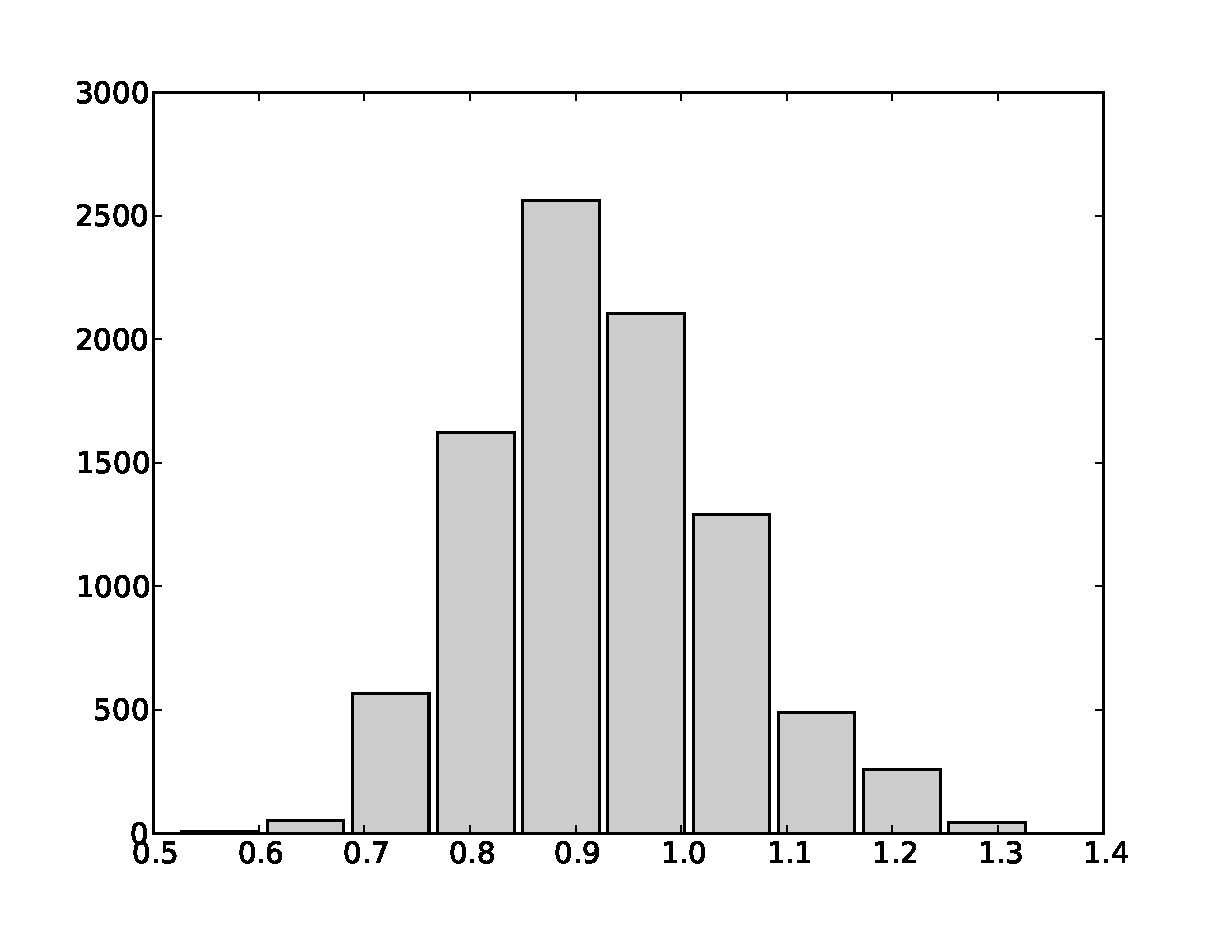
\epsfig{file=ltrace.pdf, width=10cm}
\end{center}
PyMC has its own plotting functionality, via the optional
\module{matplotlib} module as noted in the installation notes. The
\module{Matplot} module includes a \code{plot} function that takes the
model (or a single parameter) as an argument:
\begin{verbatim}
   >>> from pymc.Matplot import plot
   >>> plot(M)
\end{verbatim}
For each variable in the model, \code{plot} generates a composite figure, such as this one for the switchpoint in the disasters model:
\begin{center}
   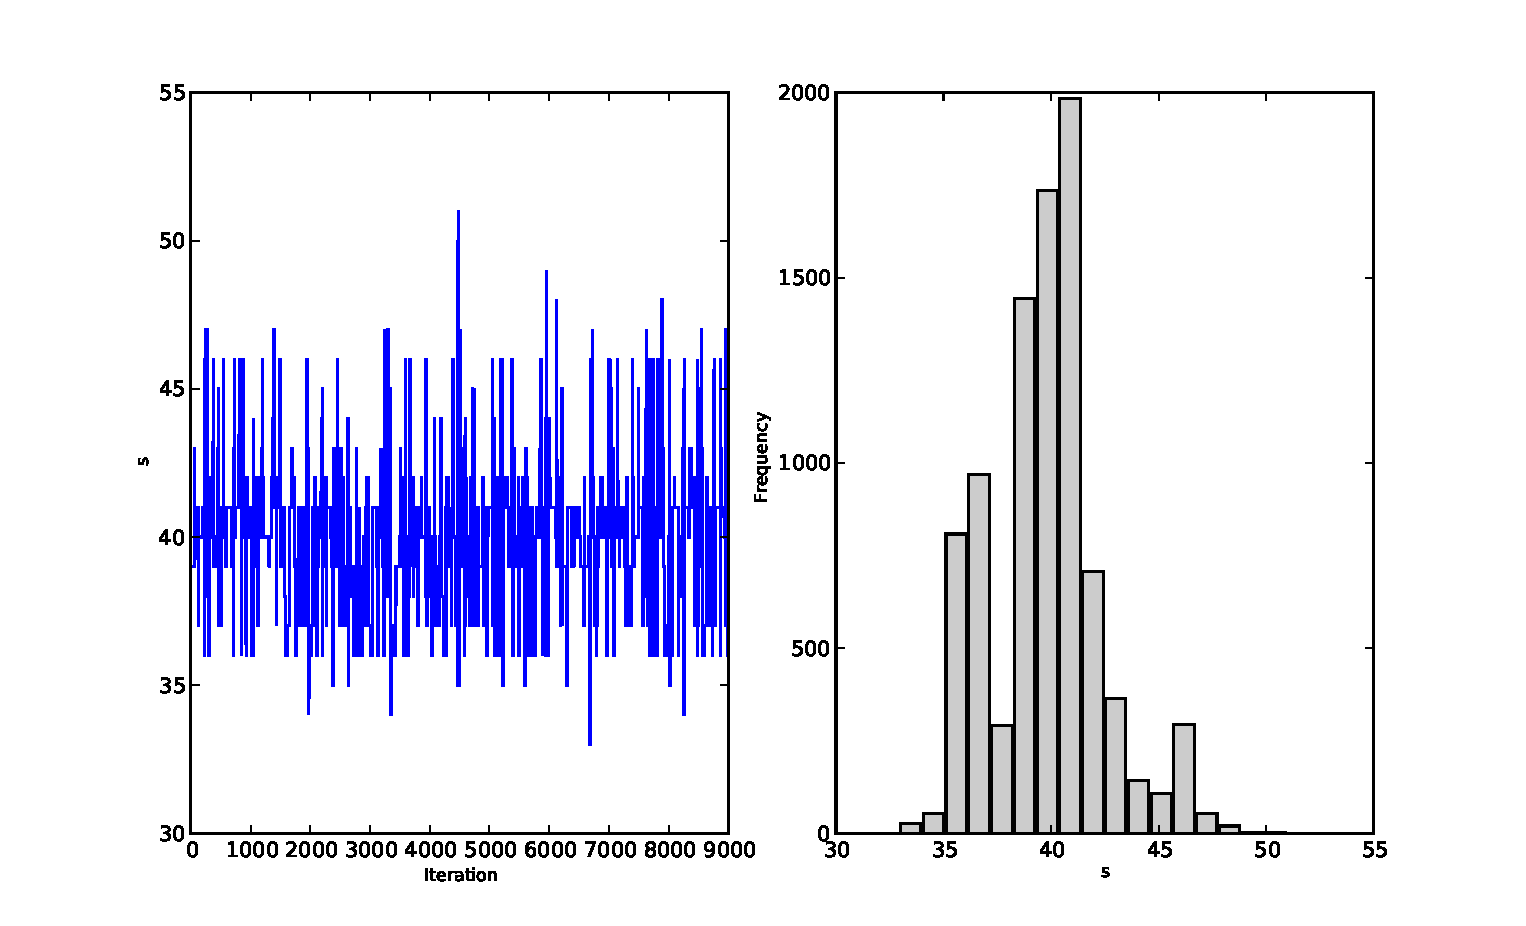
\epsfig{file=spost.pdf, width=15cm}
\end{center}
The left-hand pane of this figure shows the temporal series of the samples from $s$, while the right-hand pane shows a histogram of the trace. The trace is useful for evaluating and diagnosing the algorithm's performance (see \cite*{gelman}), while the histogram is useful for visualizing the posterior.

For a non-graphical summary of the posterior, simply call \code{M.stats()}.

\hypertarget{missing}{}
\subsection{Imputation of Missing Data} % (fold)
\pdfbookmark[1]{Imputation of Missing Data}{missing}
%\label{subsec:missing_data}

As with most ``textbook examples", the models we have examined so far assume that the associated data are complete. That is, there are no missing values corresponding to any observations in the dataset. However, many real-world datasets contain one or more missing values, usually due to some logistical problem during the data collection process. The easiest way of dealing with observations that contain missing values is simply to exclude them from the analysis. However, this results in loss of information if an excluded observation contains valid values for other quantities, and can bias results. An alternative is to impute the missing values, based on information in the rest of the model.

For example, consider a survey dataset for some wildlife species:

\begin{center}
\begin{tabular}{cccc}
\hline
Count & Site & Observer & Temperature\\
\hline
15 & 1 & 1 & 15\\
10 & 1 & 2 & NA\\
6 & 1 & 1 & 11\\
\hline
\end{tabular}
\end{center}

Each row contains the number of individuals seen during the survey, along with three covariates: the site on which the survey was conducted, the observer that collected the data, and the temperature during the survey. If we are interested in modelling, say, population size as a function of the count and the associated covariates, it is difficult to accommodate the second observation because the temperature is missing (perhaps the thermometer was broken that day). Ignoring this observation will allow us to fit the model, but it wastes information that is contained in the other covariates.

In a Bayesian modelling framework, missing data are accommodated simply by treating them as unknown model parameters. Values for the missing data $\tilde{y}$ are estimated naturally, using the posterior predictive distribution:

\begin{equation}
	p(\tilde{y}|y) = \int p(\tilde{y}|\theta) f(\theta|y) d\theta
\end{equation}

This describes additional data $\tilde{y}$, which may either be considered unobserved data or potential future observations. We can use the posterior predictive distribution to model the likely values of missing data.

Consider the coal mining disasters data introduced previously. Assume that two years of data are missing from the time series; we indicate this in the data array by the use of an arbitrary placeholder value, None.

\begin{verbatim}
x = np.array([ 4, 5, 4, 0, 1, 4, 3, 4, 0, 6, 3, 3, 4, 0, 2, 6,
3, 3, 5, 4, 5, 3, 1, 4, 4, 1, 5, 5, 3, 4, 2, 5,
2, 2, 3, 4, 2, 1, 3, None, 2, 1, 1, 1, 1, 3, 0, 0,
1, 0, 1, 1, 0, 0, 3, 1, 0, 3, 2, 2, 0, 1, 1, 1,
0, 1, 0, 1, 0, 0, 0, 2, 1, 0, 0, 0, 1, 1, 0, 2,
3, 3, 1, None, 2, 1, 1, 1, 1, 2, 4, 2, 0, 0, 1, 4,
0, 0, 0, 1, 0, 0, 0, 0, 0, 1, 0, 0, 1, 0, 1])
\end{verbatim}

To estimate these values in PyMC, we generate a masked array. These are specialised NumPy arrays that contain a matching True or False value for each element to indicate if that value should be excluded from any computation. Masked arrays can be generated using NumPy's \code{ma.masked_equal} function:
\begin{verbatim}
>>> masked_data = np.ma.masked_equal(x, value=None)
>>> masked_data
masked_array(data = [4 5 4 0 1 4 3 4 0 6 3 3 4 0 2 6 3 3 5 4 5 3 1 4 4 1 5 5 3
 4 2 5 2 2 3 4 2 1 3 -- 2 1 1 1 1 3 0 0 1 0 1 1 0 0 3 1 0 3 2 2 0 1 1 1 0 1 0
 1 0 0 0 2 1 0 0 0 1 1 0 2 3 3 1 -- 2 1 1 1 1 2 4 2 0 0 1 4 0 0 0 1 0 0 0 0 0 1
 0 0 1 0 1],
 mask = [False False False False False False False False False False False False
 False False False False False False False False False False False False
 False False False False False False False False False False False False
 False False False  True False False False False False False False False
 False False False False False False False False False False False False
 False False False False False False False False False False False False
 False False False False False False False False False False False  True
 False False False False False False False False False False False False
 False False False False False False False False False False False False
 False False False],
      fill_value=?)

\end{verbatim}

This masked array, in turn, can then be passed to PyMC's own \code{Impute} function, which replaces the missing values with Stochastic variables of the desired type. For the coal mining disasters problem, recall that disaster events were modelled as Poisson variates:

\begin{verbatim}
	>>> from pymc import Impute
	>>> D = Impute('D', Poisson, masked_data, mu=r)
	>>> D
	[<pymc.distributions.Poisson 'D[0]' at 0x4ba42d0>,
	 <pymc.distributions.Poisson 'D[1]' at 0x4ba4330>,
	 <pymc.distributions.Poisson 'D[2]' at 0x4ba44d0>,
	 <pymc.distributions.Poisson 'D[3]' at 0x4ba45f0>,
	...
	 <pymc.distributions.Poisson 'D[110]' at 0x4ba46d0>]
\end{verbatim}

Here $r$ is an array of means for each year of data, allocated according to the location of the switchpoint. Each element in $D$ is a Poisson Stochastic, irrespective of whether the observation was missing or not. The difference is that actual observations are data Stochastics (\code{observed=True}), while the missing values are non-data Stochastics. The latter are considered unknown, rather than fixed, and therefore estimated by the MCMC algorithm, just as unknown model parameters.

In this example, we have manually generated the masked array for illustration. In practice, the \code{Impute} function will mask arrays automatically, replacing all \code{None} values with Stochastics. Hence, only the original data array needs to be passed.

The entire model looks very similar to the original model:

\begin{verbatim}
	# Switchpoint
	s = DiscreteUniform('s', lower=0, upper=110)
	# Early mean
	e = Exponential('e', beta=1)
	# Late mean
	l = Exponential('l', beta=1)

	@deterministic(plot=False)
	def r(s=s, e=e, l=l):
	    """Allocate appropriate mean to time series"""
	    out = np.empty(len(disasters_array))
	    # Early mean prior to switchpoint
	    out[:s] = e
	    # Late mean following switchpoint
	    out[s:] = l
	    return out

	# Where the value of x is None, the value is taken as missing.
	D = Impute('D', Poisson, x, mu=r)
\end{verbatim}

\begin{figure}[ht]
\begin{center}
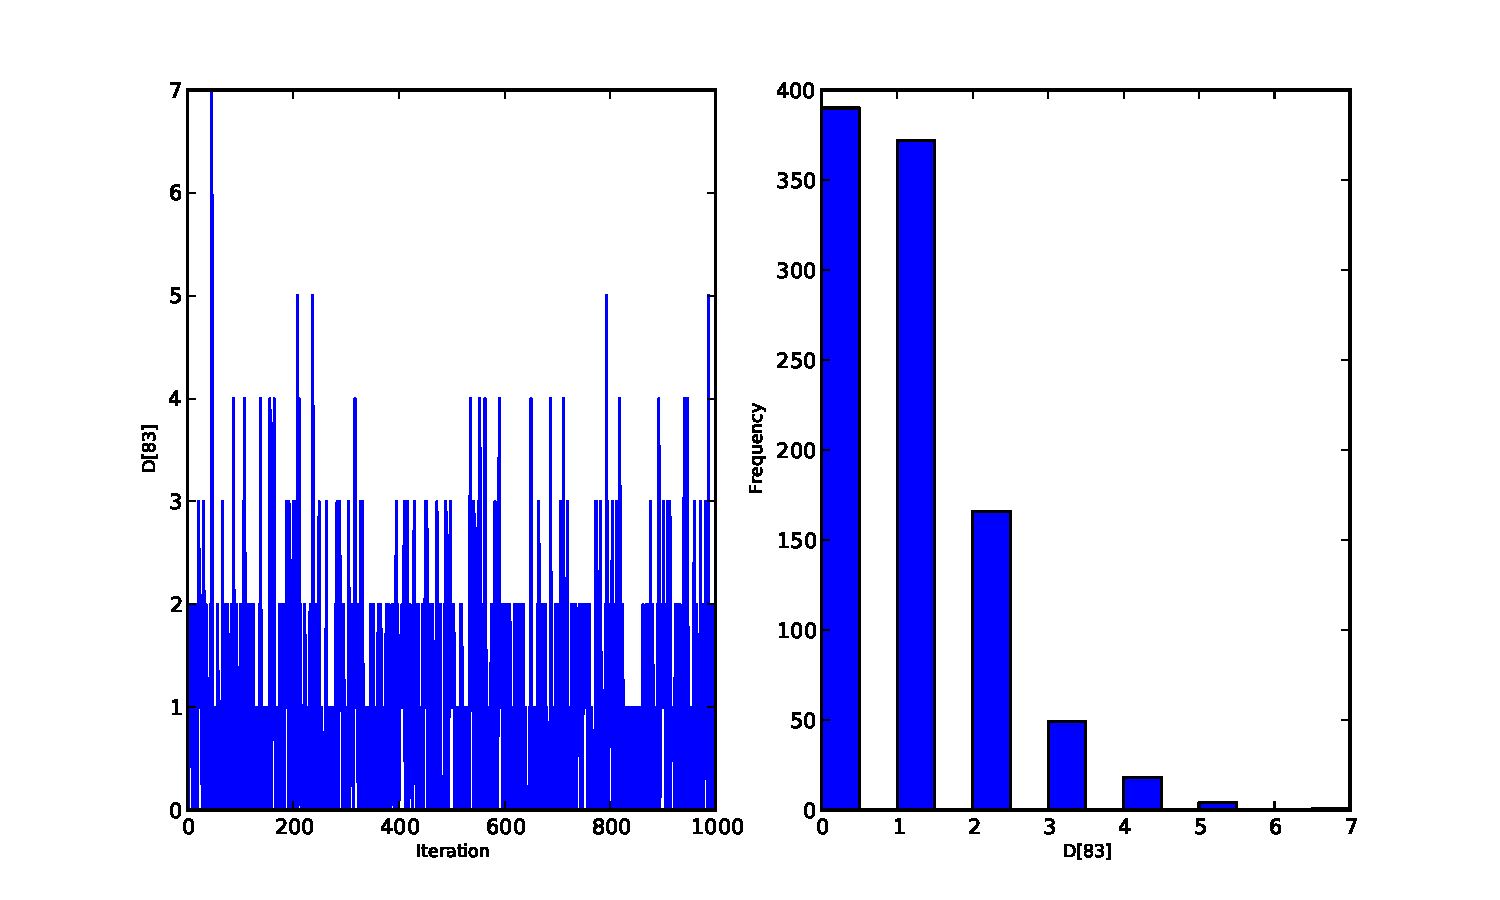
\includegraphics[height=3in]{missing.pdf}
\caption{Trace and posterior distribution of the second missing data point in the example.}
\label{fig:missing}
\end{center}
\end{figure}


The main limitation of this approach for imputation is performance. Because each
element in the data array is modelled by an individual Stochastic, rather than a
single Stochastic for the entire array, the number of nodes in the overall model
increases from 4 to 113. This significantly slows the rate of sampling, due to
the overhead costs associated with iterations over individual nodes.

% section missing_data (end)


\section{Fine-tuning the MCMC algorithm}

MCMC objects handle individual variables via \emph{step methods}, which determine how parameters are updated at each step of the MCMC algorithm. By default, step methods are automatically assigned to variables by PyMC. To see which step methods $M$ is using, look at its \code{step_method_dict} attribute with respect to each parameter:
\begin{verbatim}
   >>> M.step_method_dict[DisasterModel.s]
   >>> [<pymc.StepMethods.DiscreteMetropolis object at 0x3e8cb50>]

   >>> M.step_method_dict[DisasterModel.e]
   >>> [<pymc.StepMethods.Metropolis object at 0x3e8cbb0>]

   >>> M.step_method_dict[DisasterModel.l]
   >>> [<pymc.StepMethods.Metropolis object at 0x3e8ccb0>]
\end{verbatim}
The value of \code{step_method_dict} corresponding to a particular variable is a list of the step methods $M$ is using to handle that variable.

You can force $M$ to use a particular step method by calling \code{M.use_step_method} before telling it to sample. The following call will cause $M$ to handle $l$ with a standard \code{Metropolis} step method, but with proposal standard deviation equal to $2$:
\begin{verbatim}
   >>> from pymc import Metropolis
   >>> M.use_step_method(Metropolis, DisasterModel.l, proposal_sd=2.)
\end{verbatim}

Another step method class, \code{AdaptiveMetropolis}, is better at handling highly-correlated variables. If your model mixes poorly, using \code{AdaptiveMetropolis} is a sensible first thing to try.



\section{Beyond the basics}
That was a brief introduction to basic PyMC usage. Many more topics are covered in the subsequent sections, including:
\begin{itemize}
   \item Class \code{Potential}, another building block for probability models in addition to \code{Stochastic} and \code{Deterministic}
   \item Normal approximations
   \item Using custom probability distributions
   \item Object architecture
   \item Saving traces to the disk, or streaming them to the disk during sampling
   \item Writing your own step methods and fitting algorithms.
\end{itemize}
Also, be sure to check out the documentation for the Gaussian process extension,
which is available on PyMC's
\href{http://code.google.com/p/pymc/downloads/list}{download} page.
